% Modified from ICML 2012 example latex template

% Use the following line _only_ if you're still using LaTeX 2.09.
%\documentstyle[icml2012,epsf,natbib]{article}
% If you rely on Latex2e packages, like most moden people use this:
\documentclass[english]{article}

% For figures
\usepackage{graphicx} % more modern
%\usepackage{epsfig} % less modern
\usepackage{subfigure} 

% For citations
\usepackage{natbib}

% For algorithms
\usepackage{algorithm}
\usepackage{algorithmic}

% As of 2011, we use the hyperref package to produce hyperlinks in the
% resulting PDF.  If this breaks your system, please commend out the
% following usepackage line and replace \usepackage{icml2012} with
% \usepackage[nohyperref]{icml2012} above.
\usepackage{hyperref}

\usepackage{bbm}
\usepackage{pbox}
\usepackage{babel}
\usepackage{enumitem}

% Packages hyperref and algorithmic misbehave sometimes.  We can fix
% this with the following command.
\newcommand{\theHalgorithm}{\arabic{algorithm}}

% Employ the following version of the ``usepackage'' statement for
% submitting the draft version of the paper for review.  This will set
% the note in the first column to ``Under review.  Do not distribute.''
% \usepackage{icml2012} 
% Employ this version of the ``usepackage'' statement after the paper has
% been accepted, when creating the final version.  This will set the
% note in the first column to ``Appearing in''
\usepackage[accepted]{icml2012}


% The \icmltitle you define below is probably too long as a header.
% Therefore, a short form for the running title is supplied here:
% \icmltitlerunning{Submission and Formatting Instructions for ICML 2012}

\begin{document} 

\twocolumn[
\icmltitle{Predicting Time Spent with Physician}

\icmlauthor{Jim Zheng}{jimzheng@stanford.edu}
\icmladdress{Stanford University, Computer Science Dept., 353 Serra Mall, Stanford, CA 94305 USA}
\icmlauthor{Ioannis (Yannis) Petousis}{petousis@stanford.edu\ }
\icmladdress{Stanford University, Electrical Engineering Dept., 353 Serra Mall, Stanford, CA 94305 USA}
\icmlauthor{Ye (Scott) Cheng}{scottcheng@stanford.edu\ }
\icmladdress{Stanford University, Computer Science Dept., 353 Serra Mall, Stanford, CA 94305 USA}

\vskip 0.3in
]


\begin{abstract}
The goal of this project is to predict how much time a physician should be spending with a patient, given the patient's injury, referral status, and other reported, non-identifiable medical information.
This may be used as an additional factor for measuring and predicting physician efficiency alongside existing methodology.
We implement linear regression and a variety of classification techniques on a national dataset of Emergency Room (ER) patients and outpatients.
We use cross validation to select the optimum set of features.
In addition, we implement the k-Means algorithm to generate new features for our supervised learning algorithms.
Our final models provide good predictions of time spent with physician with a mean error of around 7 minutes.
\end{abstract}


\section{Introduction}

Current literature on measuring clinical efficiency measure cost and patient feedback efficiency, both of which have been shown to be correlated with a patient's length of stay \cite{kroch2007hospital}.
Among the many subdivisions of the length of stay, one of the most important for quality patient care is how much time a patient spends with a physician. 
Techniques in current literature for predicting length of stay include multi-label, multi-class for supervised learning.
Specifically, length of stay is transformed into a binary labeling of ``short'' or ``long'' with the separation between ``short'' and ``long'' set specific to the study \cite{snyder2010data}.
Studies also try to discretize by hourly intervals and use decision trees to discretize bins.
Existing studies do not attempt, however, to directly predict length of stay in minutes, possibly because there is no need for such precision in existing studies where the variation in length of stay is high.
The goal of our project is to predict, given a set of features that describe the circumstances of a patient visit, how much time (in minutes) a physician is likely to spend with them. 


\section{Data and Features}

Our data comes from the National Ambulatory Medical Care Survey, collected by the National Center for Health Statistics.
This annual survey samples physician-patient interactions inside hospital ER and outpatient departments across the US.
Data is collected via a predefined sampling method provided by the Center for Disease Control (CDC) that spans a wide variety of regions and clinical environments \cite{namcs2009, namcs2010}.
This is a rich dataset with over 30,000 rows per annual report (dated from 2010 back to 1992), and over 400 features recorded.

\subsection{Raw Data Structure}

Some of the features captured by the dataset include:

\begin{itemize}[noitemsep,nolistsep]
  \item age of patient
  \item day of week the appointment took place
  \item is the physician the patient's primary physician
  \item major reason for visit
  \item location (metropolitan or not, and which US region)
  \item has a computer for viewing patient info
  \item drug type prescribed
  \item patient's Body Mass Index (BMI)
\end{itemize}

It's worth noting that some of these features are continuous (age of patient, BMI), some are discrete, multivalued (day of week, drug type), and some are boolean (e.g. is primary physician).
This meant that the type of regression that we ran could operate only on a subset of all features, and extensive feature processing was necessary to obtain the best set of features.

With respect to time spent, several facts are also noteworthy.
First, time with physician is rounded to be between 0 and 240 minutes; records with times spent over 240 minutes are capped at 240.
Second, since entries are manually recorded, times are frequently arbitrarily rounded to the nearest 5 minutes.

\subsection{Preprocessing}

Data was collected by downloading and extracting a set of features listed in the documentation for each year.
Each dataset contained a slightly different set of features; this required us to search for a set of features that stayed consistent from year to year.

{\bf Binomial Smoothing:}
After running some early data analysis, we saw that quite a few features that were semantically binomial (e.g. is patient referred) were in fact represented as multinomials with values 0-9 to indicate types of errors in the recording process.
For these features, we unified error values as 0, so that 1 indicates existence, and 0 indicates that the feature was either not present or untrue for the patient.

{\bf Label smoothing:}
We also realized that the distribution of the time spent with physician field was skewed towards large values at multiples of 5 minutes, and large dropoffs for non-multiples of 5.
This reflects the fact that a good amount of time, on-the-field recording of time spent with physician is estimated and rounded to the nearest 5 minutes.
To mitigate this concern, for logistic regression, we discretize time with physician into multiples of 10 to smooth out our dataset.
We also found that more than 92\% of the data examples have one or more invalid feature values, which are generally unrecorded data.
If we include these features or training examples as they are, the invalid values would largely disturb the linear models.
We came up with two strategies to deal with this issue.
In the first approach, we take out all the examples with invalid values, and only train and test on the examples where all values are valid. This way, we make sure that all the data examples being used are real and meaningful.
In the other approach, instead of dropping invalid examples, we try to fix them by filling in the average value of the attribute over the entire dataset.
We did two things to improve the second approach. First, to ensure the representativeness of the average attribute values, we remove the features for which too many examples have invalid values. For example, if 1/5 of the examples have invalid values for a particular feature, we would not look at this feature.
Second, we remove the data examples with relatively more invalid attribute values. For example, if a data example has more than 1/15 of invalid features, we consider it as unreliable and therefore remove it from the dataset.

\subsection{Unsupervised Learning and Feature Generation}

We implemented the K-means algorithm to identify if the hospitals can be grouped into clusters based on parameters such as:

\begin{itemize}[noitemsep,nolistsep]
  \item geographical region
  \item public or private practice
  \item percentage of income derived from the state / research institutions / private insurance / patient payments
  \item the provision of electronic billing and electronic prescriptions. 
\end{itemize}

The number of centroids was varied and the total error (i.e. the sum of euclidean distances of each example from its closest centroid) was calculated. We found that $K=6$ and above gives a low error.
We will subsequently try to define new features by calculating the euclidean distance of a new training example from each of the clusters. The new features will be fed to the supervised learning algorithms.

\subsection{Principal Component Analysis}

The Principal Component Analysis (PCA) algorithm was used to exploit any dependencies in the input data by projecting them on a lower dimensional space (the number of dimensions was varied).
They were then fed into the supervised learning algorithms and the predictive performance was compared to that with the original data.


\section{Linear Regression Models}
\label{sec/linear}

Our first approach is to apply linear regression models on our dataset to predict the time with physician.
The prediction involves the following steps:

\begin{enumerate}[noitemsep,nolistsep]
  \item Incorporate custom features, including non-linear transformations and features learned from K-Means
  \item Set up linear regression model
  \item Select features using the linear model
\end{enumerate}

We will now describe each step in more detail.

\subsection{Adding Custom Features}

To improve the results of linear model predictions, we added some custom features to the dataset.
The first type of custom features is non-linear transformations of continuous features.
Since linear regression models only look at linear relationships between the target variable and feature, in order to reflect non-linear relationships in the data in linear ways so that linear models can capture them, we apply non-linear transformations on the continuous feature values of data examples.
Specifically, for continuous features (e.g. age, height, weight), if the value is x, we add the following values as additional features to the example: $x^2$, $x^3$, $\sqrt{x}$, $\sqrt[3]{x}$.

Another class of features that we add to the data for linear models are learned from K-means clustering.
Similar method of combining supervised and unsupervised learning is adopted in previous works \cite{coates2011analysis}.
Specifically, after computing $k$ clusters out of the dataset, we add $k$ additional features to each data example, where each feature represents the example's distance to a cluster centroid.

\subsection{Linear Regression Models}

We applied four types of linear regression models: linear regression, ridge regression, lasso regression, and elastic net.
We use basic linear regression as a baseline, and try different variations to see which one fits the data best.
In particular, since there are so many features in the dataset (we use 49 features for linear regression models, which does not include custom features from non-linear transformation and K-means), chances are that not all of the features are relevant to the target variable.
Therefore we try lasso regression which predicts sparse coefficients.

In ridge regression, lasso regression and elastic net, we determine the parameters using cross validation.
For example, in ridge regression, we try to optimize $\min_w || Xw - y ||^2 + \alpha\ ||w||^2$, and we set $\alpha$ by running cross validation using ridge regression model with different values of $\alpha$ and take the optimal value.

We will see the details of how these models perform in section \ref{sec/results}.

\subsection{Feature selection}

We apply feature selection before training the linear model, which prevents overfitting and makes training and predicting faster. Specifically, we apply cross validation to determine the number of feature to maintain, and use recursive feature elimination to choose the set of features to use in our model.


\section{Classification}
\label{sec/clf}

Our second major approach for supervised learning was to discretize physician time into bins.
First, we designated a number of bins and a distribution of labels in each bin, and ran feature selection to reduce our feature set.
Next, we iteratively refined our features by smoothing, combining certain common features, and generating new ones via unsupervised learning techniques to get better predictions.
We also experimented with other classifiers to try and eliminate feature bias.

We used the following algorithms in our analysis:
Multinomial Naive Bayes,
Weighted Logistic Regression,
Random Forest Classifier,
Forward Feature Selection,
Univariate Feature Selection (using ANOVA F-value as a scoring function).
We implemented Naive Bayes and Forward Feature Selection by ourselves using numpy. We used python’s scikit-learn library \cite{pedregosa2011scikit} for all other algorithms. Weighted logistic regression is done by scikit-learn using an One vs All (OvA) approach, rather than true multiclass logistic regression.

\subsection{Naive Bayes}

As an initial benchmark, we implemented discretized, multinomial Naive Bayes with Laplace Smoothing.
We trained our model on the 2009 dataset and tested using the 2010 dataset, and initially chose our number of bins to be 10 (i.e. our interval was 10, and ranged from 0 to 90).
Naive Bayes was quick to implement and gave us a first baseline for error.
Moreover, the Naive Bayes assumption is a fair assumption to make for a large subset of our features, since the dataset combines patient, physician, region, and facility information, all of which are expected to be weakly correlated.
For discretized Naive Bayes, our approach can approximate the use of the true probability density function given the appropriate selection of interval and number of classes contained in each interval \cite{yang2009discretization}.

Naive Bayes yielded poor initial performance ($accuracy < 0.03$) on the initial set of features for the 2009 dataset; predictions were skewed right, even though the dataset was skewed left.
Using feature selection eliminated the ``drugtype'' features, which, when included, were responsible for the right bias.
Our own implementation of forward feature selection (selecting $N=10$ features) produced an accuracy of about 0.28.
We suspected that this had to do with a latent bias in the features we were selecting for. To test this suspicion, we ran scikit-learn’s Random Forest Classifier on the initial set of features and produced an accuracy score of 0.28.
This prompted us to focus on feature generation as a next step in improving classification accuracy.

\subsection{Feature Generation and Error Analysis}

Since initial benchmarks gave rather poor performance, we attempted to gain better insight into the features. We found that many features were unable to distinguish between multiple labeling, since there was much noise. Thus, we eliminated these features altogether. Next, since we were uncertain about the target number of features for forward feature selection, we opted for filter feature selection using the ANOVA F-test statistic as our scoring function. Using this type of feature selection, we reduced our analysis down to only four features. Feeding this narrowed feature set into Naive Bayes boosted our accuracy to 0.49, and random forests accuracy to 0.48.

Residual analysis showed we were predicting only three distinct intervals: 10-20, 50-60, and 70-80 bucket. This meant that we were mispredicting the 0-10, 20-30, and 30-40, which accounted for about 43\% of our data. Here, we tried a combination of techniques to reduce this bias and boost accuracy with varying degrees of success:

{\bf Combining binary features:}
We tried to combine several features into a binomial feature in order to create better separation of labelings among our feature set. This boosted our accuracy by 0.02.

{\bf Combine train and testing dataset:}
In an effort to reduce randomization, we combined the 2009 and 2010 datasets into one dataset, and randomly chose a 70-30 split for our training and testing datasets, respectively. This yielded a change in accuracy of about 0.01 on average, depending on the permutation.

{\bf Weighted logistic regression:}
Logistic regression was tried with class weights of {10: 0.5, $\langle rest \rangle$: 1}, in an effort to reduce overfitting to the 10-20 bucket. This decreased accuracy by about 0.05, as true positives with the 10-20 labeling were now being mispredicted.

{\bf Binary Labeling:}
Our final attempt was to discretize times into only two buckets, and by hour, according to existing literature. Using these weaker predictions, we were predictably able to improve our performance to over 98\% accuracy with labelings.


\section{Results}
\label{sec/results}

This section discusses our results from both linear regression models and classification models. As a baseline, in our dataset, if we predict all the data examples using the mean of target variable, the resulting mean absolute error (MAE) is 8.17 minutes.

\begin{table}
\centering
  \begin{tabular}{|l|c|c|}
  \hline
  Include K-means features  & Include & Not include \\
  \hline
  Linear Regression & 7.20                   & 7.29                        \\
  \hline
  Ridge Regression  & 7.07                   & 7.22                       \\
  \hline
  \end{tabular}
\caption{Linear regression models: MAE (minutes) from 10-fold cross validation (K=50)}
\label{tab/linres}
\end{table}

% \begin{figure}[ht]
% % \vskip 0.2in
% \begin{center}
% \centerline{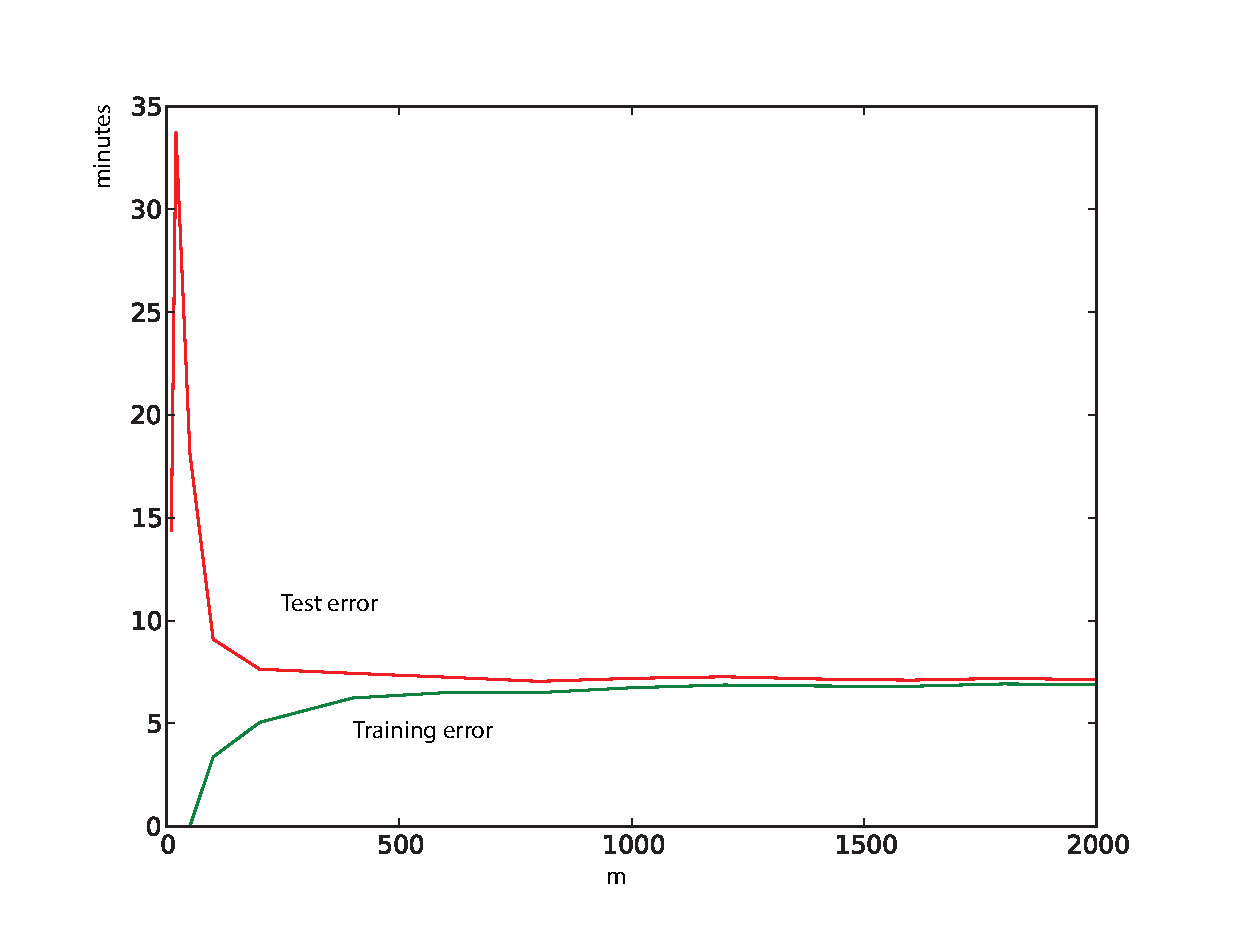
\includegraphics[width=\columnwidth]{linreg_tte}}
% \caption{}
% \end{center}
% % \vskip -0.2in
% \end{figure} 

\begin{figure*}[!htb]
\minipage{0.32\textwidth}
  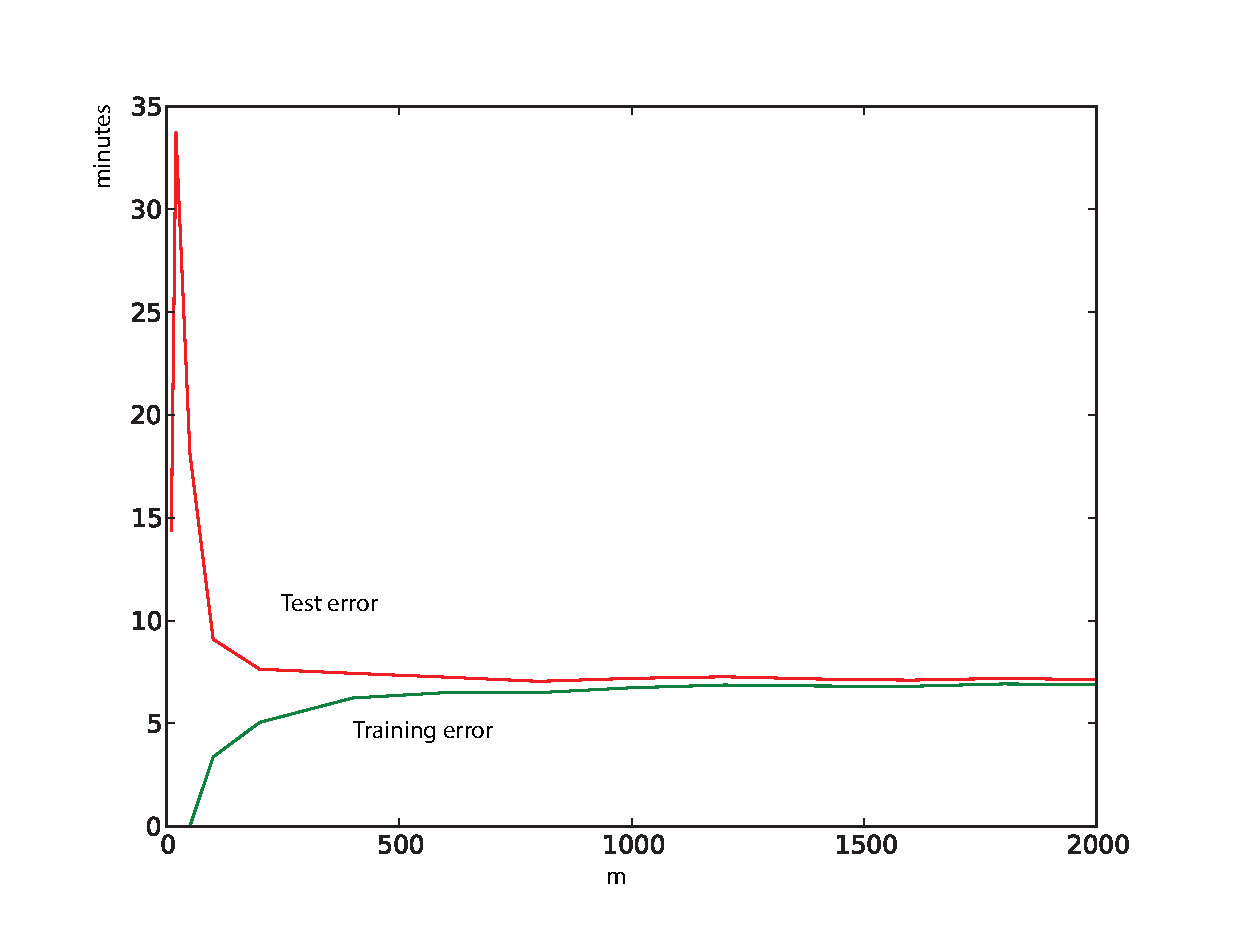
\includegraphics[width=\linewidth]{linreg_tte}
  \caption{Ridge regression: training error and test error over m\\}
\endminipage\hfill
\minipage{0.32\textwidth}
  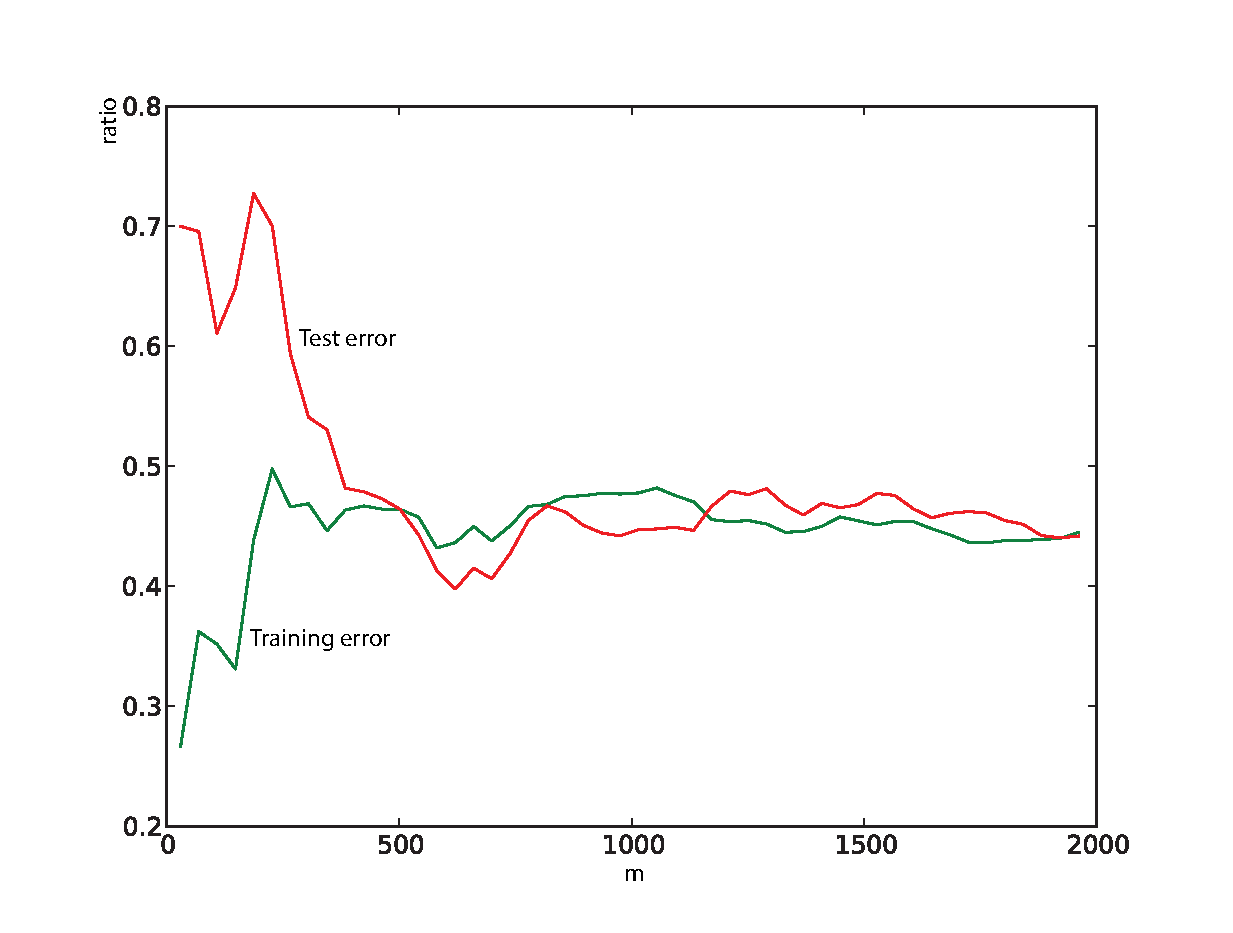
\includegraphics[width=\linewidth]{nb_tte_accuracy}
  \caption{Multinomial Naive Bayes: training error and test error over m in terms of accuracy}
\endminipage\hfill
\minipage{0.32\textwidth}%
  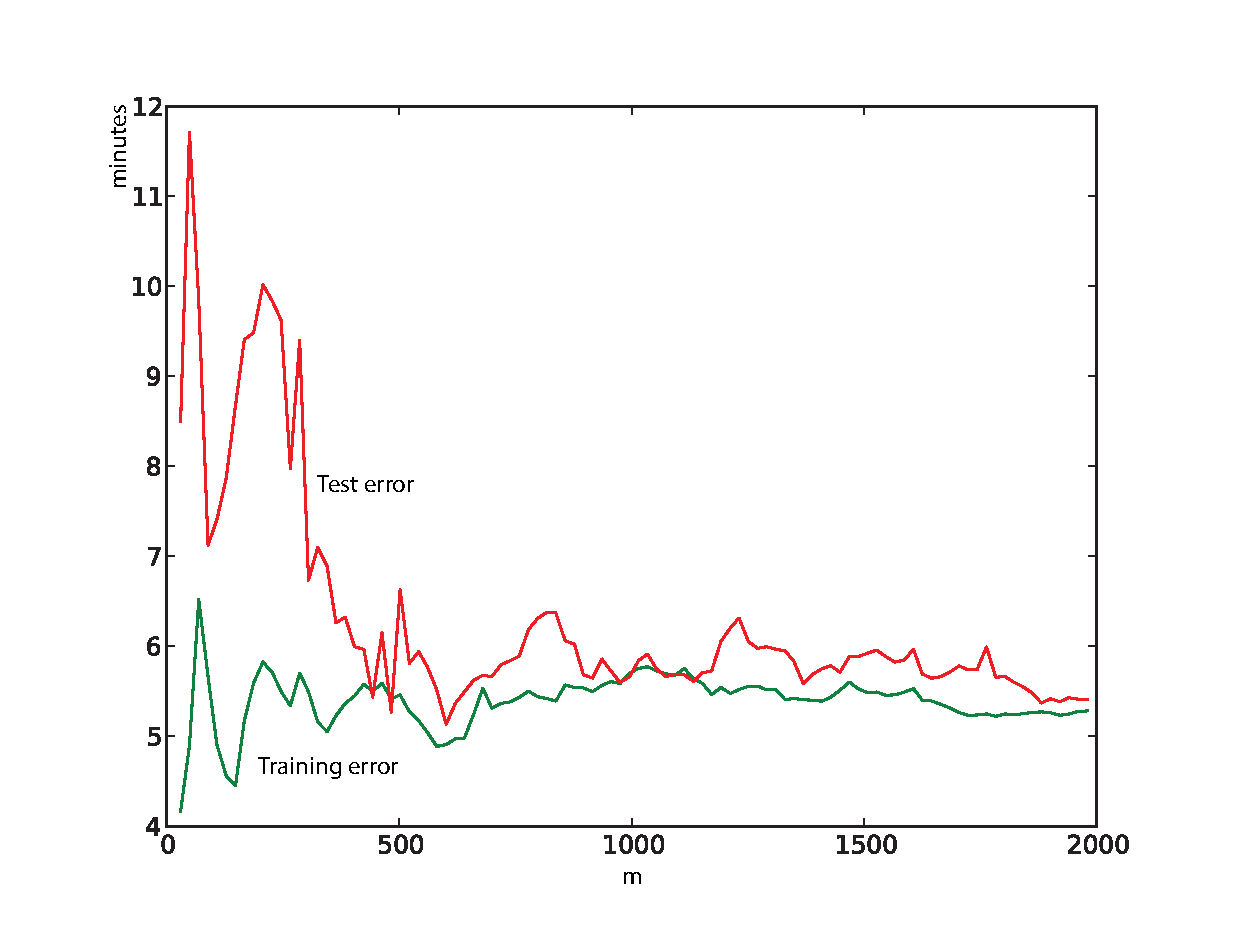
\includegraphics[width=\linewidth]{nb_tte}
  \caption{Multinomial Naive Bayes: training error and test error over m in terms of MAE}
\endminipage
\end{figure*}

\subsection{Linear Regression Models Results}

Linear regression models are able to make predictions with an MAE of around 7.1 minutes. We now discuss the different parameters and factors that affect the performance of linear regression models.

We first compare the performance of different linear models.
Lasso regression and elastic net try to establish the model on fewer features. While we initially thought this could work well since our data has a large number of features, not all of which are directly relevant to the target variable, it turns out that lasso regression and elastic net yield poor performance.
For the other two linear regression models we tried, ridge regression produces better results than linear regression.

We found that including features learned from K-means dramatically improves the performance of linear regression. The improvement is particularly significant when K is relatively large. Table \ref{tab/linres} compares the results with features learned from K-means and the results without these features.

\subsection{Classification Results}

Table \ref{tab/clf} compares the results of different classification models, where bucket size is set to 10 minutes. As mentioned in section \ref{sec/clf}, increasing bucket size will significantly improve classification accuracy, but we are more interested in more fine-grained predictions.

\begin{table}[h]
\centering
  \begin{tabular}{|l|c|c|}
  \hline
  ~    & Accuracy & MAE \\
  ~    & (percent) & (minutes)  \\
  \hline
  \ Multinomial NB & 48.5                  & 7.30                        \\
  \hline
  \ Random Forest  & 47.8                   & 7.56                       \\
  \hline
  \ Logistic Regression  & 47.6                   & 7.38                       \\
  \hline
  \end{tabular}
\caption{Classification: Accuracy and MAE}
\label{tab/clf}
\end{table}

For classification, it was difficult to see how accuracy correlated with strength of prediction for a continuous variable. We wanted to see, for example, whether our classifier made lots of mispredictions that were off by 10 and a few off by 80 vs consistently off by 20. We thus used MAE as a metric of performance in classification:

$$
\frac{1}{m}\sum_{i=1}^{m} \mathbbm{1}\{\hat{y}_i \neq y_i\}(E[\hat{y}_i] - y_i)
$$

In addition, we assume a roughly Gaussian distribution over the bins, which is a roughly good approximation since most data points are concentrated in multiples of 10; thus, the expectation is the mean of the bin.


\section{Conclusion and Future Work}

Our study represents a first attempt at directly trying to predict ``time spent with physician'', to minutes accuracy.
Our attempts at making stronger predictions with linear regression yielded an average error that was better than the average error obtained from predicting the mean.
In addition, if we weaken our predictions to match those found in current literature, we are able to obtain over 98\% accuracy in classifying time spent with physician. 

Further studies could continue improving upon our classification and regression techniques by investigating the following:

{\bf Interval and Interval Distribution Selection:}
We experimented with several interval numbers of varying weakness.
The weakest we tried was 5 minutes' intervals, the most 60 (hourly).
We also tried to restrain and randomly sample examples that fell into each bucket to ensure an even distribution.
A more principled approach would have automated over a range of possible intervals and samplings and calculated scorings for each pair of (interval, sampling).

% {\bf Multi-label classification:}
% An alternative set of labelings worthy of investigation is the office setting (clinical/mental institution/private practice, etc. see Appendix \ref{appendix/office}).
% Turning our classification problem into a multi-label, multi-class problem (predicting a pairing of (time class, label)) could potentially yield better and more interesting results when segregating by office setting in addition to time spent with physician.

{\bf Training on larger dataset}
At the time of testing, we were unable to access documentation for the datasets starting from 2003 to 2008, which prevented us from gathering more training data. Using more training data could potentially improve our linear regression predictions; since our linear regression model eliminated mostly-null rows and thus had only about 10\% of the original training set with which to train.


\nocite{pope2007health}

\bibliography{cs229}
\bibliographystyle{icml2012}

% \appendix
% \section{Types of Office Settings}
% \label{appendix/office}

% \begin{enumerate}
%   \item Private Solo or Group Practice
%   \item Free Standing Clinics
%   \item Community Health Center
%   \item Mental Health Center
%   \item Non federal governmental clinic
%   \item Family planning clinic
%   \item HMO (Health Maintenance Organization)
%   \item Faculty Practice Plan
% \end{enumerate}

\end{document} 
